\documentclass{myclass}

\begin{document}

\section{Wnioskowanie Bayesowskie}

Typowym sposobem połączenia wyników matematycznej teorii prawdopodobieństwa z eksperymentami jest
interpretacja częstościowa, która stwierdza iż prawdopodobieństwo zdarzenia \(A\) to częstość
realizacji \(A\) w dużej liczbie prób. Dla wielu zdarzeń pojęcie \emph{dużej liczby prób} nie jest
jednak dobrze zdefiniowane. Wówczas interpretacja Bayesowska prawdopodobieństwa jako miary
niepewności co do rezultatu określonego zdarzenia jest bardziej naturalna. Wnioskowanie Bayesowskie
opiera się na twierdzeniu Bayesa 
\[
\boxed{
\underbrace{p(\bm{x} \mid \bm{y})}_{\text{posterior}} = \frac{ \underbrace{p(\bm{y} \mid \bm{x})}_{\text{likelihood}} \underbrace{p(\bm{x})}_{\text{prior}}}{\underbrace{\int p(\bm{y} \mid \bm{x}) p(\bm{x}) \dd{\bm{x}}}_{\text{evidence}}}
}
\]
oraz dwóch regułach znanych z rachunku prawdopodobieństwa: \emph{sum rule} i \emph{product rule}.
\[
    p(\bm{x}) = \int p(\bm{x}, \bm{y}) \dd{\bm{y}} \,,\quad p(\bm{x}, \bm{y}) = p(\bm{x} \mid \bm{y}) p(\bm{y})\,.
\]
Typowe zastosowanie wnioskowania Bayesowskie przebiega następująco: mamy pewien zbiór obserwacji
\(\mc{X}\), o których zakładamy, iż pochodzą z pewnego rozkładu prawdopodobieństwa z parametrami
\(\bm{\theta}\), tj. znamy wiarygodność \(p(\mc{X} \mid \bm{\theta})\). Zakładamy dodatkowo pewien
prior nad parametrami \(p(\bm{\theta})\). Następnie korzystając z twierdzenia Bayesa wyznaczamy
rozkład a posteriori nad parametrami modelu
\[
    p(\bm{\theta} \mid \mc{X}) = \cfrac{p(\mc{X} \mid \bm{\theta}) p(\bm{\theta})}{ \displaystyle \int p(\mc{X} \mid \bm{\theta}) p(\bm{\theta}) \dd{\bm{\theta}}} \,.
\]
Rozkład a posteriori podsumowuje całą naszą wiedzę o estymowanym parametrze (z perspektywy
wnioskowania Bayesowskiego). Korzystając z tego rozkładu możemy:
\begin{itemize}
    \item Wyznaczyć estymatę punktową (tzw. estymatę \emph{maximum a posteriori} (MAP)) parametru
    \(\bm{\theta}\) jako
    \[
    \boxed{
        \bm{\theta}_\text{MAP} = \argmax_{\bm{\theta}} p(\bm{\theta} \mid \mc{X})
    }\quad.
    \]

    \item Wyznaczyć \emph{przedział wiarygodności} (ang. \emph{credible interval}, nie mylić z
    przedziałem ufności) parametru \(\bm{\theta}\) jako
    \[
        C_\alpha (\bm{\theta}; \mc{X}) = (\underline{\bm{\theta}}, \overline{\bm{\theta}})\,,
    \]
    gdzie
    \[
        \int\limits_{\underline{\bm{\theta}}}^{\overline{\bm{\theta}}} p(\bm{\theta} \mid \mc{X}) \dd{\bm{\theta}} = 1 - \alpha\,.
    \]

    \item Skonstruować \emph{rozkład predyktywny} (ang. \emph{posteriori predictive distribution})
    dla nowych obserwacji
    \[
    \boxed{
        p(\bm{x} \mid \mc{X}) = \int p(\bm{x} \mid \bm{\theta}) p(\bm{\theta} \mid \mc{X}) \dd{\bm{\theta}}
    }\quad.
    \]

    \item Możemy wyznaczyć wartość parametru \(\bm{\theta}\), która minimalizuje oczekiwaną stratę
    dla pewnej funkcji kosztu
    \[\begin{split} \bm{\theta}^* &= \argmin_{\bm{\theta}'} \Ebb_{\bm{\theta} \sim
        p(\bm{\theta}\mid\mc{X})}\left[ L(\bm{\theta}', \bm{\theta}) \right] \\
                      &= \argmin_{\bm{\theta}'} \int L(\bm{\theta}, \bm{\theta}') p(\bm{\theta} \mid
                      \mc{X}) \dd{\bm{\theta}}\,.
    \end{split}
    \]

\end{itemize}

\section{Rozkład normalny}

Wielowymiarowy rozkład normalny o średniej \(\bm{\mu} \in \Rbb^n\) i symetrycznej, nieujemnie
określonej macierzy kowariancji \(\bm{\Sigma} \in \Rbb^{n \times n}\) to rozkład o gęstości danej
przez
\[
    p(\bm{x} \mid \bm{\mu}, \bm{\Sigma}) = \frac{1}{\displaystyle (2\pi)^\frac{n}{2} |\bm{\Sigma}|^\frac{1}{2}} \exp \left[-\frac{1}{2} (\bm{x} - \bm{\mu})^\tpose \bm{\Sigma}^{-1} (\bm{x} - \bm{\mu})\right]\,.
\]
Macierz \(\bm{\Lambda} = \bm{\Sigma}^{-1}\) nazywamy macierzą precyzji. Będziemy często korzystać z
następującej własności rozkładów normalnych: jeśli zmienne \(\bm{x} \in \Rbb^n\) i \(\bm{y} \in
\Rbb^m\) mają łącznie wielowymiarowy rozkład normalny
\[
    \mqty[\bm{x} \\ \bm{y}] \sim \mc{N}\left(\mqty[\bm{\mu}_x \\ \bm{\mu}_y], \mqty[\bm{\Sigma}_{xx} & \bm{\Sigma}_{xy} \\ \bm{\Sigma}_{yx} & \bm{\Sigma}_{yy}]\right)\,,
\]
to rozkłady brzegowe są rozkładami normalnymi
\[
    \bm{x} \sim \mc{N}(\bm{\mu}_x, \bm{\Sigma}_{xx})\,,\quad \bm{y} \sim \mc{N}(\bm{\mu}_y, \bm{\Sigma}_{yy})
\]
oraz rozkłady warunkowe są rozkładami normalnymi
\[
    \bm{x} \mid \bm{y} \sim \mc{N}(\bm{\mu}_{x\mid y}, \bm{\Sigma}_{x \mid y})\,,
\]
gdzie
\[
\begin{split}
    &\bm{\mu}_{x \mid y} = \bm{\mu}_x + \bm{\Sigma}_{xy} \bm{\Sigma}_{yy}^{-1} (\bm{y} - \bm{\mu}_y) \\
    &\bm{\Sigma}_{x \mid y} = \bm{\Sigma}_{xx} - \bm{\Sigma}_{xy} \bm{\Sigma}_{yy}^{-1} \bm{\Sigma}_{yx}
\end{split}\quad.
\]

\section{Liniowe modele Gaussowskie}

Jednym z najprostszych modeli, do którego można zastosować wnioskowanie Bayesowskie jest tzw.
liniowy model Gaussowski. Zakładamy, iż mamy obserwację \(\bm{y}\), która pochodzi z rozkładu
normalnego
\[
    \bm{y} \mid \bm{x} \sim \mc{N}(\bm{A}\bm{x} + \bm{b}, \bm{\Sigma}_y)\,,
\]
gdzie \(\bm{x}\) jest pewną zmienną ukrytą (ang. \emph{hidden variable}), natomiast \(\bm{A}\),
\(\bm{b}\) i \(\bm{\Sigma}_y\) są znane dokładnie. Dodatkowo przyjmijmy \emph{prior sprzężony do
wiarygodności} dla parametru \(\bm{x}\) będący rozkładem normalnym o znanych parametrach
\(\bm{\mu}_x\), \(\bm{\Sigma}_x\)
\[
    \bm{x} \sim \mc{N}(\bm{\mu}_x, \bm{\Sigma}_x) \,.
\]
Wówczas rozkład a posteriori również będzie rozkładem normalnym o parametrach
\[
\begin{split}
    &\bm{\mu}_{x \mid y} = \bm{\Sigma}_{x \mid y} \left( \bm{A}^\tpose \bm{\Sigma}_y^{-1}(\bm{y} - \bm{b}) + \bm{\Sigma}_x^{-1} \bm{\mu}_x \right)\\
    &\bm{\Sigma}_{x \mid y} = \left(\bm{\Sigma}_x^{-1} + \bm{A}^\tpose \bm{\Sigma}_y^{-1} \bm{A} \right)^{-1}
\end{split}\quad.
\]

\section{Regresja liniowa}

Załóżmy, że modelujemy obserwacje postaci \((y, \bm{x})\), gdzie \(y\) to skalar zwany \emph{zmienną
objaśnianą}, natomiast \(\bm{x}\) to wektor cech lub inaczej \emph{zmiennych objaśniających}.
Zakładamy, że zmienna objaśniana zależy liniowo od zmiennych objaśniających oraz, iż zależność ta
jest obarczona pewnym błędem losowym. Model ten ma więc postać
\[
\boxed{
    y(\bm{x}) = \phi(\bm{x}; \bm{w}, b) + \epsilon = \bm{w}^\tpose \bm{x} + b + \epsilon\,,
}
\]
gdzie \(y(\bm{x})\) jest wartością zmiennej losowej obserwowaną dla znanego dokładnie wektora cech
\(\bm{x}\) (wektor cech \emph{nie} jest zmienną losową), natomiast \(\bm{w}\) i \(b\) to parametry
modelu \(\phi\), o których chcemy wnioskować. Model ten jest typowym przykładem \emph{regresji
liniowej}. Parametryzację regresji liniowej można uprościć przyjmując, że do wektora cech dokładamy
stałą wartość \(1\), a parametr \(b\) włączamy do \(\bm{w}\)
\[
    \bm{x}^\tpose \gets \mqty[\bm{x}^\tpose & 1]\,,\quad \bm{w}^\tpose \gets \mqty[\bm{w}^\tpose & b] \,.
\]
W zależności od przyjętego rozkładu zmiennej opisującej błąd losowy \(\epsilon\) otrzymujemy różne
modele, np.:
\begin{itemize}
    \item regresja liniowa (ang. \emph{linear regression}), \(\epsilon \sim \mc{N}(0, \sigma^2)\)
    dla znanego \(\sigma^2\),

    \item regresja odporna (ang. \emph{robust regression}), \(\epsilon \sim \text{Laplace}(0,
    \lambda)\) dla znanego \(\lambda\)
    \[
        \text{Laplace}(x; \mu, \lambda) = \frac{1}{2b} \exp\left[- \frac{|x - \mu|}{b}\right]\quad,
    \]
    \item regresja kwantylowa (ang. \emph{quantile regression}), \(\epsilon \sim \text{ALD}(0,
    \lambda, p)\) dla znanego \(\lambda\) i percentyla \(p\)
    \[
        \text{ALD}(x; \mu, \lambda, p) = \frac{p(1-p)}{\lambda} \cdot \begin{cases}
                \displaystyle \e^{-\frac{(p-1)(x-\mu)}{\lambda}} &\,, x \leq \mu\\
                \displaystyle \e^{-\frac{p (x - \mu)}{\lambda}}  &\,, x > \mu
        \end{cases}.
    \]  
\end{itemize}

Zauważmy tutaj, że założenie iż znamy skalę (tj. parametry \(\sigma\), \(\lambda\)) błędu jest dosyć
mocne -- z reguły nie wiemy jak dokładnie możemy przybliżyć zmienną objaśnianą. Dokładne
wnioskowanie Bayesowskie przeprowadzimy tylko dla pierwszego z powyższych modeli, gdzie błędy mają
rozkład normalny. To założenie, choć sensowne, ma również swoje konsekwencja -- nasz model będzie
dosyć wrażliwy na obserwacje odstające (ang. \emph{outliers}). Zamiast rozkładu normalnego można
przyjąć rozkład, w którym gęstość prawdopodobieństwa ma tzw. ciężkie ogony (ang. \emph{heavy tails})
-- np. rozkład Laplace'a. Otrzymamy wówczas model zwany odporną regresją liniową (ang. \emph{robust
linear regression}). Oba powyższe modele równo rozkładają masę prawdopodobieństwa błędów. Jeśli
interesuje nas natomiast estymacja kwantyli warunkowych (tj. prostej która najlepiej dzieli
obserwacje tak aby odpowiedni ułamek z nich znalazł się pod nią), to możemy wykorzystać asymetryczny
rozkład Laplace'a. Otrzymany model nazywamy wówczas kwantylową regresją liniową (ang. \emph{quantile
linear regression}).

Przyjmijmy obecnie, że dysponujemy zbiorem obserwacji \(\mc{X} = \{(y_i, \bm{x}_i)\}_{i=1}^n\).
Zakładamy, że obserwacje te są i.i.d. -- niezależne i pochodzące z tego samego rozkładu \(y_i \sim
\mc{N}(\phi(\bm{x}_i; \bm{w}), \sigma^2)\). Jawne wnioskowanie Bayesowskie możliwe jest również dla
regresji liniowej. Bardzo często jednak stosuje się prostsze podejście adekwatne również do
pozostałych dwóch modeli. Otóż poszukujemy jedynie estymaty punktowe parametrów \(\bm{w}\),
ignorując niepewność ich oszacowania. Taką estymację punktową można wyznaczyć \emph{metodą
największej wiarygodności} (ang. \emph{maximum likelihood estimation} (MLE))
\[
\boxed{
    \bm{w}_\text{MLE} = \argmax_{\bm{w}} p(\mc{X} \mid \bm{w})
}\,.
\]
Korzystamy wówczas jedynie z wiarygodności \(p(\mc{X} \mid \bm{w})\). Z założenia, iż obserwacje są
i.i.d. możemy łatwo wyznaczyć wiarygodność
\[
\begin{split}
    p(\mc{X} \mid \bm{w}) &= \prod_{i=1}^n \mc{N}(y_i; \phi(\bm{x}_i; \bm{w}), \sigma^2) \\
                          &\propto \prod_{i=1}^n \exp\left(-\frac{(y_i - \phi(\bm{x}_i; \bm{w}))^2}{2\sigma^2}\right)\,,
\end{split}
\]
gdzie pominęliśmy współczynnik, gdyż nie ma on wpływu na zagadnienie optymalizacji. W praktyce
często łatwiej jest minimalizować sumę pewnych wyrażeń, niż ich iloczyn, dlatego wprowadzamy
\emph{zanegowaną logarytmiczną funkcję wiarygodności} (ang. \emph{negated log-likelihood function}
(NLL))
\[
\boxed{
    L(\mc{X}, \bm{w}) = - \log p(\mc{X} \mid \bm{w})
}\,,
\]
gdzie korzystamy oczywiście z faktu, iż logarytm (naturalny) jest funkcją ściśle rosnącą. Estymatę
MLE możemy wówczas znaleźć jako
\[
\boxed{
    \bm{w}_\text{MLE} = \argmin_{\bm{w}} L(\mc{X}, \bm{w})
}\,.
\]
W przypadku regresji liniowej otrzymujemy
\[
    \bm{w}_\text{MLE} = \argmin_{\bm{w}} \frac{1}{2}\sum_{i=1}^n (y_i - \phi(\bm{x}_i; \bm{w}))^2\,.
\]
Z powyższego problemu optymalizacyjnego wynika popularna nazwa tej formy regresji liniowej --
\emph{metoda najmniejszych kwadratów} (ang. \emph{Ordinary Least Squares} (OLS)), ponieważ
minimalizujemy sumę kwadratów rezyduów. W tym szczególnym przypadku postać \(\bm{w}_\text{MLE}\)
można znaleźć analitycznie. Istotnie wprowadźmy
\[
    \bm{y} = \mqty[y_1 \\ \vdots \\ y_n]\,,\quad \bm{X} = \mqty[\bm{x}_1^\tpose \\ \vdots \\ \bm{x}_n^\tpose]\,,\quad \bm{\phi} = \bm{X}\bm{w}\,.
\]
Wówczas mamy
\[
    \pdv{L}{\phi_\beta} = (\phi_\beta - y_\beta)
\]
oraz dalej
\[
    \pdv{L}{w_\alpha} = \sum_{\beta=1}^n \pdv{L}{\phi_\beta} \pdv{\phi_\beta}{w_\alpha} = \sum_{\beta=1}^n (\phi_\beta - y_\beta) X_{\beta\alpha}\,.
\]
Z warunków koniecznych dla minimum lokalnego mamy \(\forall \alpha : \pdv{L}{w_\alpha} = 0\), co
możemy zapisać jako
\[
    \bm{X}^\tpose(\bm{\phi} - \bm{y}) = \bm{X}^\tpose(\bm{X}\bm{w}_\text{MLE} - \bm{y}) = \bm{0}\,,
\]
skąd
\[
    \bm{w}_\text{MLE} = (\bm{X}^\tpose \bm{X})^{-1} \bm{X}^\tpose \bm{y}\,.
\]
Wielkość \((\bm{X}^\tpose \bm{X})^{-1} \bm{X}^\tpose\) nazywa się pseudo odwrotnością
Moore'a--Penrose macierzy \(\bm{X}\). Warto tutaj zaznaczyć, iż w praktyce rzadko wyznaczamy
\(\bm{w}_\text{MLE}\) korzystając wprost z powyższego wzoru, ze względu na dość słabe własności
numeryczne. Typowo jeśli macierz \(\bm{X}\) jest niewielka, to pseudo odwrotność obliczamy
korzystając z rozkładu SVD macierzy \(\bm{X}\). Natomiast dla dużych macierzy nie korzystamy ze
wzoru analitycznego tylko z metody iteracyjnej stochastycznego spadku wzdłuż gradientu
\[
    w_\alpha^{(t+1)} = w_\alpha^{(t)} - \eta \pdv{L}{w_\alpha}\,,
\]
która w tym przypadku zbiega do minimum globalnego \(\bm{w}_\text{MLE}\).

\subsection{Regresja Bayesowska}

Pokażemy teraz, jak przeprowadzić pełne wnioskowanie Bayesowskie dla modelu regresji liniowej.
Założymy rozkład a priori nad parametrami \(\bm{w}\) w postaci rozkładu normalnego
\[
    \bm{w} \sim \mc{N}(\bm{\mu}_0, \bm{\Sigma}_0)\,.
\]
Wiarygodność, jak pokazaliśmy powyżej ma natomiast postać
\[
    \mc{X} \mid \bm{w} \sim \mc{N}(\bm{X}\bm{w}, \sigma^2 \bm{I})\,.
\]
Zauważmy, że jest to instancja modelu liniowego, więc korzystając z wyprowadzonych wzorów wiemy, iż
\[
    \bm{w} \mid \mc{X} \sim \mc{N}(\bm{\mu}_n, \bm{\Sigma}_n)\,,
\]
gdzie
\[
\begin{split}
    &\bm{\mu}_n = \bm{\Sigma}_n\left(\frac{1}{\sigma^2} \bm{X}^\tpose \bm{y} + \bm{\Sigma}_0^{-1}\bm{\mu}_0 \right)\\
    &\bm{\Sigma}_n = \left(\bm{\Sigma}_0^{-1} + \frac{1}{\sigma^2} \bm{X}^\tpose \bm{X} \right)^{-1}
\end{split}\,.
\] 
W powyższych wzorach nazwy parametrów nie są przypadkowe. Przed zaobserwowaniem danych mamy rozkład
a priori \(\bm{w} \mid \mc{N}(\bm{\mu}_0, \bm{\Sigma}_0)\). Po zaobserwowaniu \(n\) przykładów
aktualizujemy nasze przekonania w postaci rozkładu a posteriori \(\bm{w} \mid \mc{X} \sim
\mc{N}(\bm{\mu}_n, \bm{\Sigma}_n)\).

Znając rozkład a posteriori nad \(\bm{w}\) możemy również wyznaczyć rozkład predykcyjny nad zmienną
objaśnianą \(y\) dla ustalonego wektora cech \(\bm{x}\). Formalnie interesuje nas rozkład \(p(y \mid
\mc{X})\). Rozkład ten możemy opisać w następujący sposób
\[
\begin{split}
    &\bm{w} \mid \mc{X} \sim \mc{N}(\bm{\mu}_n, \bm{\Sigma}_n)\\
    &y \mid \bm{w} \sim \mc{N}(\bm{w}^\tpose \bm{x}, \sigma^2)
\end{split}
\]
gdzie interesuje nas rozkład
\[
    p(y \mid \mc{X}) = \int p(y \mid \bm{w}) p(\bm{w} \mid \mc{X}) \dd{\bm{w}}\,.
\]
Można pokazać, iż rozkład ten jest rozkładem normalnym
\[
    y \mid \mc{X} \sim \mc{N}(\mu_y, \sigma_y^2)
\]
o parametrach
\[
    \mu_y = \bm{\mu}_n^\tpose \bm{x}\,,\quad \sigma^2_y = \sigma^2 + \bm{x}^\tpose \bm{\Sigma}_n \bm{x}\,.
\]

\subsection{Regresja grzbietowa}

Rozważmy Bayesowską regresję liniową, w której prior ma postać \(\bm{w} \sim \mc{N}(0,
\tau^2\bm{I})\), czyli elementy wektora parametrów są a priori wzajemnie niezależne a ich amplitudy
są rzędu \(\tau\). Znajdźmy estymatę MAP parametrów \(\bm{w}\). Zauważmy, że 
\[
-\log p(\bm{w} \mid \mc{X}) \propto \left[ \frac{1}{2\sigma^2}\sum_{i=1}^n (y_i - \phi(\bm{x}_i; \bm{w}))^2 + \frac{1}{2\tau^2}\norm{\bm{w}}_2^2 \right]\,. 
\]
Wyrażenie w nawiasach możemy przemnożyć przez \(\sigma^2\) -- nie wpłynie to na położenie minimum,
bo \(\sigma^2\) to dodatnia stała. Estymata MAP w tym modelu to zatem
\[
    \bm{w}_\text{MAP} = \argmin_{\bm{w}} \left[ \frac{1}{2}\sum_{i=1}^n (y_i - \phi(\bm{x}_i; \bm{w}))^2 + \frac{\gamma}{2}\norm{\bm{w}}_2^2 \right]
\]
gdzie \(\gamma = \sigma^2 / \tau^2\) to \emph{stała regularyzująca}. Pierwszy z członów to znana z
OLS suma kwadratów rezyduów, natomiast drugi człon to \emph{człon regularyzujący} rozwiązanie, który
ogranicza amplitudy parametrów (wag). Jest to tzw. model \emph{regresji grzbietowej} (ang.
\emph{ridge regression}). Jest to jednocześnie oczywiście moda rozkładu a posteriori, czyli w
przypadku rozkładu normalnego -- wyznaczony wcześniej parametr \(\bm{\mu_n}\)
\[
    \bm{w}_\text{MAP} = \left(\frac{\sigma^2}{\tau^2}\bm{I} + \bm{X}^\tpose\bm{X}\right)^{-1}\bm{X}^\tpose\bm{y}\,.
\]

\subsection{*Regresja w ujęciu częstościowym}

Podstawowym pytaniem, na które sama estymacja punktowa nie daje odpowiedzi w przypadku modelu
liniowego jest: czy dany podzbiór współczynników jest istotny statystycznie? Oczywiście w ujęciu
Bayesowskim odpowiedzi na to pytanie udziela rozkład a posteriori nad parametrami modelu. Chcemy
mieć jednak również klasyczną, częstościową argumentację. Niech \(\hat{y}_i\) będzie odpowiedzą
modelu dla cech \(\bm{x}_i\), a \(y_i\) prawdziwą odpowiedzią. Wielkość
\[
    \text{RSS} := \sum_{i=1}^N (y_i - \hat{y}_i)^2
\]
nazywamy \emph{rezydualną sumą kwadratów} (ang. \emph{residual sum of squares}). Wówczas jeśli
potrzebujemy testu sprawdzającego istotność podzbioru współczynników tzn. testujemy hipotezę
\[
    H_0 : w_{i_1} = 0\,,\ldots\,,w_{i_q} = 0
\]
to odpowiednią statystyką testową jest 
\[
    \frac{ \text{RSS}_0 -  \text{RSS}}{ \text{RSS}}\frac{n - p - 1}{q} \sim F(q, n-p-1)\,,
\]
gdzie \( \text{RSS}_0\) oznacza rezydualną sumę kwadratów dla modelu spełniającego \(H_0\), \(F\) oznacza
rozkład F Snedecora, natomiast \(p\) to liczba wszystkich parametrów modelu.

Korzystając z metod częstościowych możemy również podać przedział ufności na poziomie \(1 - \alpha\)
przy przewidywaniu odpowiedzi dla nieznanej wartości \(\bm{x}_0\) jako
\[
    \bm{\hat{w}}^\tpose \bm{x}_0 \pm t_{1-\frac{\alpha}{2},n-p-1} \hat{\sigma}^2 \sqrt{\bm{x}_0^\tpose \left(\bm{X}^\tpose \bm{X}\right)^{-1}\bm{x}_0}\,,
\]
gdzie
\[
    \hat{\sigma}^2 = \frac{ \text{RSS}}{n - p - 1}
\]
natomiast \(t_{1-\frac{\alpha}{2},n-p-1}\) jest kwantylem rzędu \(1-\frac{\alpha}{2}\) rozkładu t
Studenta z parametrem \(n - p - 1\).

\begin{figure}[ht]
    \centering
    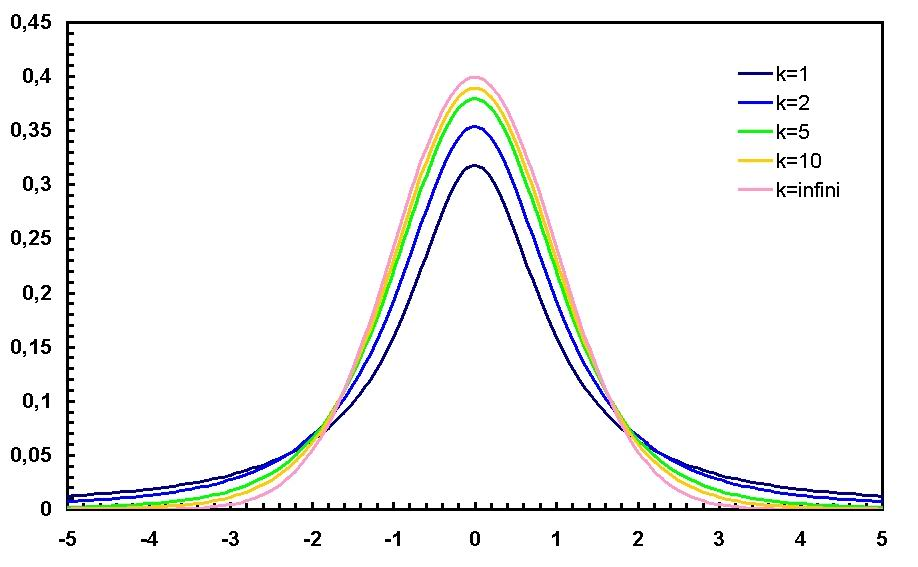
\includegraphics[width=0.85\columnwidth]{figs/Student_densite_best.jpeg}
\end{figure}


\subsection{Uogólnione Modele Liniowe}

W uogólnionym modelu liniowym zakładamy, że \(y(\bm{x})\) ma rozkład pochodzący z ustalonej
\emph{wykładniczej rodziny rozkładów o nadmiernej dypsersji} \(p(\cdot; \theta(\bm{x}), \tau)\) z
parametrem \(\theta(\bm{x})\) i znanym \(\tau\). Natomiast parametr \(\theta(\bm{x})\) rozkładu
\(y(\bm{x})\) jest związany ze składnikiem systematycznym równością
\[
    \mu\left( \Ebb[y(\bm{x})]\right) = \bm{w}^\tpose \bm{x}
\]
dla pewnej \emph{funkcji wiążącej} (ang. \emph{link function}) \(\mu\).

Wykładniczą rodziną rozkładów z nadmierną dyspersją z parametrami \(\theta\), \(\tau\) nazywa się
rodzinę rozkładów, których gęstości (lub funkcje) prawdopodobieństwa mają postać
\[
    p(x; \theta, \tau) = \exp\left(\frac{\theta x - F(\theta)}{d(\tau)} + k(x,\tau)\right)\,,
\]
gdzie \(F\), \(d\) i \(k\) to pewne funkcje. Można wówczas pokazać, że jeśli \(X \sim p(x; \theta,
\tau)\), to
\[
    \Ebb[X] = F'(\theta)\,,\quad \mathbb{V}[X] = F''(\theta)d(\tau)\,.
\]
Rodzinami wykładniczymi są:
\begin{itemize}
    \item \(\mc{N}(m, \sigma^2)\) dla \(\theta =m\) i \(\tau = \sigma^2\),
    \item \(\text{Bin}(n,p)\) z ustaloną liczbą prób \(n\) dla \(\theta = \text{logit}(p)\) i \(\tau
    = 1\),
    \item \(\text{Pois}(\lambda)\) dla \(\theta = \log \lambda\) i \(\tau = 1\).
\end{itemize}
Rodzinami wykładniczymi nie są np. \(t_\nu\) i \(\mc{U}(a,b)\) z nieustalonymi końcami przedziału.


\section{Wprowadzenie do procesów Gaussowskich}

Macierz kowariancji \(n\)--wymiarowej zmiennej losowej \(\bm{x}\) o wartości oczekiwanej
\(\bm{\mu}\) jest zdefiniowana jako
\[
\bm{\Sigma} = \mathbb{E}\left[(\bm{x} - \bm{\mu})(\bm{x} - \bm{\mu})^\tpose\right]\,.
\]
Wiemy również, iż macierz ta jest nieujemnie określona. Pokażemy teraz, iż dla każdej nieujemnie
określonej macierzy symetrycznej \(\bm{K}\) wymiaru \(n\times n\) istnieje \(n\)--wymiarowa zmienna
losowa o wielowymiarowym rozkładzie normalnym, dla której \(\bm{K}\) jest macierzą kowariancji.
Istotnie dla każdej nieujemnie określonej macierzy symetrycznej istnieje macierz \(\bm{L}\) taka, że
\[
\bm{K} = \bm{L}\bm{L}^\tpose\,,
\]
jest to tzw. \emph{dekompozycja Choleskiego}. Niech \(\bm{z} \sim \mc{N}(\bm{0}, \bm{1})\), wówczas
zmienna losowa \(\bm{L}\bm{z}\) ma rozkład o zerowej wartości oczekiwanej i macierzy kowariancji
\[
\mathbb{E}\left[(\bm{L}\bm{z})(\bm{L}\bm{z})^\tpose\right] = \bm{L}\mathbb{E}[\bm{z}\bm{z}^\tpose]\bm{L}^\tpose = \bm{L}\bm{1}\bm{L}^\tpose = \bm{K}\,.
\]
Powyższe własności wskazują, iż macierze kowariancji można w pewnym sensie utożsamiać z nieujemnie
określonymi macierzami symetrycznymi.

Funkcję \(k: \mathbb{R}^n\times\mathbb{R}^n\mapsto\mathbb{R}\) taką, że \(\forall m\in\mathbb{N} :
\forall X = \{\bm{x}_1,\ldots,\bm{x}_m\} \subset \mathbb{R}^n\) macierz
\[
k(X,X) = \mqty[k(\bm{x}_1, \bm{x}_1) & k(\bm{x}_1, \bm{x}_2) & \cdots & k(\bm{x}_1, \bm{x}_m)\\
k(\bm{x}_2, \bm{x}_1) & k(\bm{x}_2, \bm{x}_2) & \cdots & k(\bm{x}_2, \bm{x}_m)\\
\vdots & \vdots & \ddots & \vdots\\
k(\bm{x}_m, \bm{x}_1) & k(\bm{x}_m, \bm{x}_2) & \cdots & k(\bm{x}_m, \bm{x}_m)\\]
\]
jest dodatnio określoną macierzą symetryczną nazywamy funkcją kowariancji, jądrem dodatnio
określonym (ang. \emph{positive definite kernel}) lub \emph{jądrem Mercera}.

Dla dwóch zbiorów punktów \(X = \{\bm{x}_1,\ldots,\bm{x}_m\} \subset \mathbb{R}^n\) i \(Y =
\{\bm{y}_1,\ldots,\bm{y}_s\} \subset \mathbb{R}^n\) i funkcji kowariancji \(k\) wprowadzimy
oznaczenie
\[
k(X,Y) := \mqty[k(\bm{x}_1, \bm{y}_1) & k(\bm{x}_1, \bm{y}_2) & \cdots & k(\bm{x}_1, \bm{y}_s)\\
k(\bm{x}_2, \bm{y}_1) & k(\bm{x}_2, \bm{y}_2) & \cdots & k(\bm{x}_2, \bm{y}_s)\\
\vdots & \vdots & \ddots & \vdots\\
k(\bm{x}_m, \bm{y}_1) & k(\bm{x}_m, \bm{y}_2) & \cdots & k(\bm{x}_m, \bm{y}_s)\\]\,.
\]
Poniżej podajemy kilka przykładów funkcji kowariancji
\begin{itemize}
    \item \emph{Gaussian kernel} dla normy \(\norm{\cdot}\) i hiper-parametrów \(a,l\) (amplituda i
    skala długości)
    \[
    k(\bm{x}, \bm{y}) = a^2\exp\left\{-\frac{1}{2l^2}\norm{\bm{x} - \bm{y}}^2\right\}
    \]
    
    \item \emph{Periodic kernel} dla normy \(\norm{\cdot}\) i hiper-parametrów \(a, l, p\)
    (amplituda, skala długości, okres zmienności)
    \[
    k(\bm{x},\bm{y}) = a^2\exp\left\{-\frac{2}{l^2}\sin^2\left(\frac{\pi}{p}\norm{\bm{x} - \bm{y}}\right)\right\}
    \]
    
    \item \emph{White noise kernel} dla hiper-parametru \(\sigma\)
    \[
    k(\bm{x},\bm{y}) = \sigma^2 \delta_{\bm{x},\bm{y}}
    \]
    
    \item \emph{Mat\'ern kernel} dla normy \(\norm{\cdot}\) i hiper-parametrów \(a, l, \nu\)
    (amplituda, skala długości, regularność)
    \[
    k(\bm{x},\bm{y}) = a^2 \frac{2^{1-\nu}}{\Gamma(\nu)}\left(\frac{\sqrt{2\nu}}{l}\norm{\bm{x} - \bm{y}}\right)^\nu K_\nu\left(\frac{\sqrt{2\nu}}{l}\norm{\bm{x} - \bm{y}}\right)\,,
    \]
    gdzie \(\Gamma(x)\) to funkcja gamma Eulera, a \(K_\nu(x)\) to zmodyfikowana funkcja Bessela
    2-go rodzaju rzędu \(\nu\).

\end{itemize}
Suma lub iloczyn dwóch funkcji kowariancji oraz złożenie funkcji kowariancji z wielomianem o
nieujemnych współczynnikach jest również funkcją kowariancji

Procesem Gaussowskim (ang. \emph{Gaussian Process}) nazywamy rodzinę skalarnych zmiennych losowych
indeksowanych przez punkty \(\bm{x} \in \mathbb{R}^n\)
\[
\mc{GP} = \left\{f_{\bm{x}} \mid \bm{x} \in \mathbb{R}^n\right\}
\]
taką że każdy skończony podzbiór \(\mc{GP}\) ma łącznie wielowymiarowy rozkład normalny tj. dla
dowolnego zbioru \(X = \{\bm{x}_1, \ldots, \bm{x}_m\} \subset \mathbb{R}^n\) zachodzi
\[
\mqty[f_{\bm{x}_1} \\ \vdots \\ f_{\bm{x}_m}] \sim \mc{N}(\bm{\mu}_X, \bm{\Sigma}_{X})\,.
\]

Zauważmy, iż proces Gaussowski możemy jednoznacznie zdefiniować podając przepisy na parametry
\(\bm{\mu}_X\) i \(\bm{\Sigma}_X\) dla dowolnego zbioru \(X\). W praktyce często przyjmujemy
\(\bm{\mu}_X = \bm{0}\), natomiast przepisem na macierz kowariancji może być zdefiniowana wyżej
funkcja kowariancji \(k(X,X)\) tj.
\[
\mqty[f_{\bm{x}_1} \\ \vdots \\ f_{\bm{x}_m}] \sim \mc{N}(\bm{0}, k(X,X))\,.
\]
Process Gaussowski daje nam w praktyce rozkład prawdopodobieństwa nad funkcjami
\(f:\mathbb{R}^n\mapsto\mathbb{R}\), których charakter jest określony przez jądro \(k\) (np. funkcja
gładka dla jądra Gaussowskiego, okresowa dla jądra periodycznego, itp.). Zauważmy, że nie
wnioskujemy tu o parametrach konkretnej rodziny funkcji (jak w przypadku regresji liniowej);
interesuje nas jedynie rozkład predykcyjny. Załóżmy, iż w dokładnie znanych przez nas punktach \(X =
\{\bm{x}_1,\bm{x}_2,\ldots,\bm{x}_m\}\) zaobserwowaliśmy wartości pewnej funkcji, o których
zakładamy, iż pochodzą z procesu Gaussowskiego zadanego jądrem \(k\), które wyraża nasze założenia a
priori co do charakteru badanej funkcji
\[
\bm{f}_X = \mqty[f_{\bm{x}_1} \\ \vdots \\ f_{\bm{x}_m}] \sim \mc{N}(\bm{0}, k(X,X))\,.
\]
Powiedzmy, iż chcemy znać wartości \(\bm{f}_Y\) tej funkcji w zadanych punktach \(Y =
\{\bm{y}_1,\bm{y}_2,\ldots,\bm{y}_s\}\). Ponieważ założyliśmy, iż wartości funkcji pochodzą z
procesu Gaussowskiego, więc rozkład łączny \(\bm{f}_X\) i \(\bm{f}_Y\) jest rozkładem normalnym
\[
\mqty[\bm{f}_X \\ \bm{f}_Y] \sim \mc{N}\left(\bm{0}, \mqty[k(X,X) & k(X,Y) \\ k(Y,X) & k(Y,Y)]\right)\,.
\]
Zauważmy, iż z twierdzenia o własnościach niezdegenerowanego rozkładu normalnego wnioskujemy, iż
warunkowy \(\bm{f}_Y\mid \bm{f}_X\) jest również rozkładem normalnym o parametrach
\[
\begin{split}
&\bm{\mu} = k(Y,X)k^{-1}(X,X)\bm{f}_X\\
&\bm{\Sigma} = k(Y,Y) - k(Y,X)k^{-1}(X,X)k(X,Y)
\end{split}\quad.
\]
Dodatkową niepewność związaną z pomiarem wartości \(\bm{f}_X\) możemy uchwycić zmieniając postać
jądra 
\[
k(\bm{x},\bm{y}) \leftarrow k(\bm{x},\bm{y}) + \mc{I}_X(\bm{x})\sigma^2\delta_{\bm{x},\bm{y}}\,,
\]
gdzie \(\sigma\) jest hiper-parametrem określającym precyzję pomiaru. Oczywiście \(k\) jest dalej
funkcją kowariancji, gdyż takie podstawienie powoduje jedynie dodanie dodatnich członów do pewnych
elementów diagonalnych macierzy kowariancji, więc macierz ta jest nadal symetryczna i dodatnio
określona. Wówczas rozkład predykcyjny ma parametry
\[
\boxed{
\begin{split}
&\bm{\mu} = k(Y,X)\left[k(X,X) + \sigma^2\bm{1}\right]^{-1}\bm{f}_X\\
&\bm{\Sigma} = k(Y,Y) - k(Y,X)\left[k(X,X) + \sigma^2\bm{1}\right]^{-1}k(X,Y)
\end{split}\quad.
}
\]

\section{Regresja logistyczna}

Rozpatrzymy teraz problem klasyfikacji binarnej z perspektywy estymacji MLE. Niech \(\mc{X} =
\{t_i(\bm{x}_i)\}_{i=1}^n\) będzie zbiorem obserwacji i.i.d., gdzie zakładamy, iż \(t \in \{0,1\}\).
Jako model statystyczny przyjmiemy, iż klasa \(t(\bm{x})\) pochodzi z rozkładu Bernoulliego z
parametrem \(\pi(\bm{x}; \bm{w})\) (prawdopodobieństwem klasy pozytywnej, gdzie \(\pi\) jest tzw.
funkcją wiążącą, ang. \emph{link function}) zależnym od estymowanych parametrów \(\bm{w}\)
\[
t_i \mid \bm{w} \sim \mathrm{Ber}(\pi(\bm{x}_i; \bm{w}))\,.
\]
W przypadku regresji logistycznej jako funkcję \(\pi(\bm{x}; \bm{w})\) przyjmiemy
\(\sigma(\phi(\bm{x}; \bm{w}))\), gdzie
\[
\sigma(z) = \frac{1}{1 + \e^{-z}}
\]
to tzw. \emph{funkcja logistyczna} (będąca szczególnym przypadkiem funkcji sigmoidalnej), natomiast
\(\phi(\bm{x}; \bm{w})\) może być dowolną funkcją wykorzystywaną do zagadnienia regresji. W
przypadku regresji logistycznej przyjmujemy prosty model liniowy
\[
\phi(\bm{x}; \bm{w}) = \bm{w}^\tpose \bm{x}\,.
\]
Zauważmy, iż taka postać uwzględnia człon stały poprzez podstawienie \(\bm{x}^\tpose \leftarrow
\mqty[\bm{x}^\tpose & 1]\). Wiarygodność dla powyższego modelu statystycznego ma postać
\[
p(\mc{X} \mid \bm{w}) = \prod_{i=1}^n \pi(\bm{x}_i;\bm{w})^{t_i} (1 - \pi(\bm{x}_i;\bm{w}))^{1 - t_i}\,,
\]
skąd funkcja NLL
\[
\boxed{
    L(\mc{X}; \bm{w}) = - \sum_{i=1}^n \left[ t_i \log \pi_i + (1 - t_i) \log (1 - \pi_i) \right]\,,
}
\]
gdzie \(\pi_i = \pi(\bm{x}_i; \bm{w})\). Taką funkcję kosztu nazywamy \emph{binarną entropią
krzyżową} (ang. \emph{ binary cross-entropy function}). Niestety dla takiej postaci funkcji kosztu
nie można znaleźć minimum w postaci analitycznej (jak zrobiliśmy w przypadku regresji liniowej),
dlatego musimy wykorzystywać algorytmy optymalizacji numerycznej, które najczęściej wykorzystują
pierwsze pochodne funkcji kosztu po parametrach. Typowo wykorzystywanym do tego celu algorytmem jest
\emph{spadek wzdłuż gradientu} (ang. \emph{gradient descent}), w którym iteracyjnie wykonujemy
\[
    \bm{w}_{t+1} = \bm{w}_t - \eta \pdv{L}{\bm{w}}\bigg|_{\bm{w}_t}\,.
\]    
\begin{figure}[ht]
    \centering
    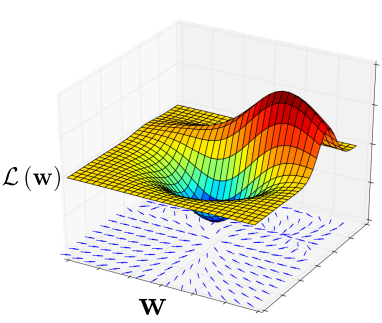
\includegraphics[width=0.85\columnwidth]{figs/image.png}
\end{figure}
Wyznaczymy więc pochodne funkcji \(L\) po parametrach \(\bm{w}\). Wprowadźmy macierz
\(X_{\alpha\beta} = x_\beta^{(\alpha)}\) oraz wektory \(\phi_\alpha = \phi(\bm{x}_\alpha; \bm{w})\),
\(\sigma_\alpha = \sigma(\phi_\alpha)\). Wówczas
\[
L(\mc{X}; \bm{w}) = - \sum_{\alpha=1}^n \left[ t_\alpha \log \sigma_\alpha + (1 - t_\alpha) \log(1 - \sigma_\alpha) \right]\,.
\]
W takim razie mamy
\[
\pdv{L}{\phi_\alpha} = \sum_{\beta=1}^n \pdv{L}{\sigma_\beta} \pdv{\sigma_\beta}{\phi_\alpha}\,,
\]
gdzie
\[
\pdv{L}{\sigma_\beta} = \frac{1 - t_\beta}{1 - \sigma_\beta} - \frac{t_\beta}{\sigma_\beta}
\]
oraz
\[
\pdv{\sigma_\beta}{\phi_\alpha} = \sigma'(\phi_\beta) \delta_{\alpha\beta}\,,
\]
gdzie
\[
\sigma'(z) = \frac{\e^{-z}}{(1 + \e^{-z})^2} = \sigma(z)(1 - \sigma(z))\,,
\]
zatem
\[
\pdv{L}{\phi_\alpha} = \left(\frac{1 - t_\alpha}{1 - \sigma_\alpha} - \frac{t_\alpha}{\sigma_\alpha}\right)\sigma_\alpha(1 - \sigma_\alpha) = \sigma_\alpha - t_\alpha\,.
\]
W takim razie, z powyższego mamy
\[
\pdv{L}{w_\alpha} = \sum_{\beta=1}^n \pdv{L}{\phi_\beta} \pdv{\phi_\beta}{w_\alpha} = \sum_{\beta=1}^n (\sigma_\beta - t_\beta) X_{\beta\alpha}\,,
\]
co możemy zapisać w zwartej postaci macierzowej
\[
\pdv{L}{\bm{w}} = \bm{X}^\tpose (\bm{\sigma} - \bm{t})\,.
\]

\section{Wieloklasowa regresja logistyczna}

Regresję logistyczną możemy w prosty sposób uogólnić na przypadek klasyfikacji jednej z \(k\) klas.
Zakładamy teraz, iż zbiór obserwacji i.i.d. ma postać \(\mc{X} = \{t_i(\bm{x}_i)\}_{i=1}^n\) dla \(t
\in \{1,\ldots,k\}\). Nasz model statystyczny uogólnimy do postaci rozkładu kategorialnego (ang.
\emph{categorical distribution} lub \emph{multinomial distribution}) z parametrem \(\bm{\pi}(\bm{x};
\bm{W})\) (wektorem prawdopodobieństw każdej klasy) zależnym od estymowanych parametrów \(\bm{W}\)
\[
t_i \mid \bm{W} \sim \mathrm{Cat}(\bm{\pi}(\bm{x}_i; \bm{W}))\,.
\]
W przypadku regresji softmax jako funkcję \(\bm{\pi}: \mathbb{R}^m \mapsto [0;1]^k\) przyjmiemy
funkcję \(\bm{\sigma}(\bm{\phi}(\bm{x}; \bm{W}))\), gdzie \(\bm{\sigma}: \mathbb{R}^k \mapsto
[0;1]^k\)
\[
\sigma_\alpha(\bm{z}) = \frac{\exp(z_\alpha)}{ \sum_{\beta=1}^k \exp(z_\beta)}
\]
to tzw. \emph{funkcja softmax}, natomiast \(\bm{\phi}: \mathbb{R}^m \mapsto \mathbb{R}^k\), to
dowolna funkcja. W przypadku regresji softmax przyjmiemy prosty model liniowy
\[
\bm{\phi}(\bm{x}; \bm{W}) = \bm{W}\bm{x}\,.
\]
Wiarygodność dla powyższego modelu ma postać
\[
\prod_{\alpha=1}^n \prod_{\beta=1}^k \pi_{\alpha\beta}^{t_{\alpha\beta}}\,,
\]
skąd funkcja NLL ma postać
\[
\boxed{
L(\mc{X}; \bm{W}) = - \sum_{\alpha=1}^n \sum_{\beta=1}^k t_{\alpha\beta} \log \pi_{\alpha\beta}\,,
}
\]
gdzie
\[
\begin{split}
    &\pi_{\alpha\beta} = \sigma_\beta(\bm{\phi}(\bm{x}_\alpha; \bm{W})) = \frac{\exp \phi_{\alpha\beta}}{\displaystyle \sum_{\gamma=1}^k \exp \phi_{\alpha\gamma}}\\
    &\phi_{\alpha\beta} = \phi_{\beta}(\bm{x}_\alpha; \bm{W}) \\
    &t_{\alpha\beta} = [t_\alpha = \beta]
\end{split}\,.
\]
Wiersze macierzy \(\bm{t}\) są binarnymi wektorami kodującymi w sposób one-hot klasę danego
przykładu. Niestety dla takiej postaci funkcji kosztu nie można znaleźć minimum w postaci
analitycznej, dlatego musimy wykorzystywać algorytmy optymalizacji numerycznej. Wyznaczymy więc
jeszcze pierwsze pochodne funkcji \(L\) po parametrach \(\bm{W}\)
\[
    \pdv{L}{\pi_{\beta\beta'}} = - \frac{t_{\beta\beta'}}{\pi_{\beta\beta'}}\,.
\]
Jednocześnie mamy
\[
    \pdv{L}{\phi_{\alpha\alpha'}} = \sum_{\beta=1}^n \sum_{\beta'=1}^k \pdv{L}{\pi_{\beta\beta'}} \pdv{\pi_{\beta\beta'}}{\phi_{\alpha\alpha'}}\,,
\]
gdzie
\[
\begin{split}
    \pdv{\pi_{\beta\beta'}}{\phi_{\alpha\alpha'}} &= \frac{\exp \phi_{\beta\beta'} \delta_{\alpha\beta} \delta_{\alpha'\beta'} }{ \displaystyle \sum_{\gamma=1}^k \exp \phi_{\beta\gamma}} - \frac{\exp \phi_{\beta\beta'} \exp \phi_{\beta\alpha'} \delta_{\alpha\beta}}{\displaystyle \left[ \sum_{\gamma=1}^k \exp \phi_{\beta\gamma} \right]^2} \\
           &= \pi_{\beta\beta'} \delta_{\alpha\beta} \delta_{\alpha'\beta'} - \pi_{\beta\beta'} \pi_{\beta\alpha'} \delta_{\alpha\beta}\,.
\end{split}
\]
Z powyższego mamy zatem
\[
    \pdv{L}{\phi_{\alpha\alpha'}} = \pi_{\alpha\alpha'} \sum_{\beta'=1}^k t_{\alpha\beta'} - t_{\alpha\alpha'} = \pi_{\alpha\alpha'} - t_{\alpha\alpha'}\,.
\]
Ostatecznie zatem
\[
    \pdv{L}{W_{\beta\beta'}} = \sum_{\alpha=1}^n \sum_{\alpha'=1}^k \pdv{L}{\phi_{\alpha\alpha'}} \pdv{\phi_{\alpha\alpha'}}{W_{\beta\beta'}}\,,
\]
gdzie
\[
    \pdv{\phi_{\alpha\alpha'}}{W_{\beta\beta'}} = X_{\alpha\beta'} \delta_{\alpha'\beta}\,,
\]
zatem
\[
    \pdv{L}{W_{\beta\beta'}} = \sum_{\alpha=1}^n (\pi_{\alpha\beta} - t_{\alpha\beta}) X_{\alpha\beta'}\,,
\]
co możemy zapisać w zwartej postaci macierzowej
\[
    \pdv{L}{\bm{W}} = (\bm{\pi} - \bm{t})^\tpose \bm{X}\,.
\]

\section{Regresja Poissonowska}
% TODO

\section{Regresja porządkowa}
% TODO

\section{Liczby losowe w komputerze}

Opiszemy teraz pokrótce metody generowania liczb pseudolosowych z dowolnych rozkładów
prawdopodobieństwa w sposób algorytmiczny. Podstawowym narzędziem, którego będziemy potrzebować do
generowania próbek z bardziej skomplikowanych rozkładów będzie prosty generator liczb z rozkładu
jednostajnego \(\mc{U}(0,1)\). Moglibyśmy oczywiście wykorzystać jakieś fizyczne urządzenie lub
proces, który generuje liczby prawdziwie losowe (np. detektor Geigera-Mullera, szum lamp
elektronowych, ruletka), ale błędem byłaby rezygnacja z odtwarzalności. Poszukujemy zatem
deterministycznej metody, która generuje sekwencje liczb, które są w przybliżeniu losowe. Podstawową
metodą do algorytmicznego generowania liczb pseudolosowych jest tzw. \emph{liniowy generator
kongruentny} (ang. \emph{Linear Congruential Generator, LCG}), który jest opisany zależnością
rekurencyjną
\[
I_{j+1} = (a I_j + c) \mod m\,,
\]
gdzie \(a, c, m\) to pewne ustalone dodatnie liczby całkowite, a \(I_0\) to tzw. ziarno (ang.
\emph{seed}). LCG generuje liczby całkowite, więc w dużym uproszczeniu liczby zmiennoprzecinkowe z
rozkładu \(\mc{U}(0,1)\) otrzymujemy jako \(I_j / m\) (trzeba tutaj jednak uwzględnić problemy
wynikające z arytmetyki zmiennoprzecinkowej).

\subsection{Metoda odwrotnej dystrybuanty}

Mając już generator liczb z rozkładu jednostajnego \(\mc{U}(0,1)\) i znając jawny wzór na
dystrybuantę \(F(x)\) innego rozkładu jednowymiarowego możemy generować liczby z tego rozkładu
korzystając z tzw. \emph{metody odwrotnej dystrybuanty}. Istotnie, jeśli \(U \sim \mc{U}(0,1)\), to
\(F^{-1}(U) \sim F\). Istotnie
\[
\Pr(F^{-1}(U) \leq x) = \Pr(U \leq F(x)) = F(x)\,.
\]
Metoda ta ma jedną zasadniczą wadę -- musimy znać jawny wzór na dystrybuantę \(F\). W przypadku np.
tak ważnych rozkładów, jak rozkład normalny dystrybuanta nie jest funkcją elementarną i metoda ta
nie jest najlepsza.

\subsection{Metoda Boxa--Mullera}

W przypadku rozkładu normalnego znacznie lepszą metodą jest tzw. \emph{metoda Boxa--Mullera}. Weźmy
rozkład łączny dwóch niezależnych zmiennych losowych \(X, Y\) pochodzących ze standardowego rozkładu
normalnego
\[
p(x, y) = \frac{1}{2\pi}\exp(\frac{1}{2}(x^2 + y^2))\,.
\]
Skorzystamy ze wzoru na transformację zmiennych losowych. Istotnie niech
\[
X = \sqrt{Z} \cos \Phi\,,\quad Y = \sqrt{Z} \sin \Phi\,,
\]
dla \(0 < Z\) oraz \( 0 \leq \Phi < 2\pi\), wówczas
\[
q(z, \phi) = \frac{1}{4\pi}\exp\frac{z}{2}\,.
\]
Zauważmy, że otrzymaliśmy sferycznie symetryczny rozkład wykładniczy. Możemy zatem wylosować kąt
\(\phi\) z rozkładu jednostajnego oraz wartość \(z\) z rozkładu wykładniczego korzystając z metody
odwrotnej dystrybuanty. Wówczas wartości \(x = \sqrt{z}\cos\phi\), \(y = \sqrt{z}\sin\phi\) będą
pochodzić ze standardowego rozkładu normalnego. Aby wygenerować próbki z ogólnego wielowymiarowego
rozkładu normalnego, korzystamy z definicji, tj. najpierw generujemy \(n\) próbek ze standardowego
rozkładu normalnego, a następnie korzystamy z przekształcenia afinicznego \(\bm{x} = \bm{A}\bm{z} +
\bm{\mu}\), gdzie \(\bm{\Sigma} = \bm{A}\bm{A}^\tpose\).

\subsection{Monte Carlo}

Umiemy już generować próbki z wielowymiarowego rozkładu normalnego. Chcemy teraz poznać metodę,
która umożliwi generowanie próbek ze skomplikowanych, wielowymiarowych rozkładów prawdopodobieństwa,
których gęstość znamy jedynie z dokładnością do stałej normalizującej, tj. znamy jedynie
\(\tilde{p}(\bm{x}) = Z p(\bm{x})\). Ograniczenie to wynika z chęci próbkowania z posteriora
\(p(\bm{x} \mid \bm{y})\) w sytuacji, gdy znamy jedynie rozkład łączny \(p(\bm{x}, \bm{y}) =
p(\bm{y} \mid \bm{x}) p_{\bm{X}}(\bm{x})\). Okazuje się, iż znajomość rozkładu jedynie z
dokładnością do stałej normalizującej jest wystarczająca do generowania próbek z tego rozkładu.
Generowanie próbek z kolei wystarcza natomiast, na mocy silnego prawa wielkich liczb, do szacowania
wartości średnich dowolnych funkcji zmiennej \(\bm{x}\). Przypomnijmy, iż na mocy silnego prawa
wielkich liczb ciąg średnich częściowych \((\overline{\bm{X}}_n)\) ciągu zmiennych losowych
\((\bm{X}_n)\) i.i.d. z rozkładu \(\bm{X} \sim \mathcal{D}\) jest zbieżny z prawdopodobieństwem 1 do
wartości oczekiwanej \(\mathbb{E}[\bm{X}]\) tj.
\[
\Pr\left(\lim_{n \to \infty} \overline{\bm{X}}_n = \mathbb{E}[\bm{X}]\right) = 1\,.
\]
Wartość oczekiwaną \(\mathbb{E}[\bm{X}]\) możemy zatem przybliżyć średnią \(\overline{\bm{X}}_n\) z
dużej ilości próbek. Poniżej przedstawimy dwa algorytmy próbkowania: algorytm IS oraz
Metropolisa--Hastingsa będący szczególną realizacją całej rodziny algorytmów próbkowania zwanych
Markov Chain Monte Carlo (MCMC).

\subsubsection{Importance sampling}

Załóżmy, iż chcemy obliczyć wartość oczekiwaną pewnej funkcji zmiennej losowej \(\bm{x}\) względem
skomplikowanego rozkładu prawdopodobieństwa \(p(\bm{x})\), który znamy jedynie z dokładnością do
stałej normalizującej
\[
p(\bm{x}) = \frac{1}{Z_p}\tilde{p}(\bm{x})
\]
tj. szukamy
\[
\mathbb{E}_{\bm{x} \sim p(\bm{x})}[f(\bm{x})] = \int f(\bm{x}) p(\bm{x})\dd\bm{x}\,.
\]
Jeśli umiemy generować próbki \(\bm{x}\) z innego (prostszego) rozkładu \(q(\bm{x})\) (np.
wielowymiarowego rozkładu normalnego), który nazywamy rozkładem proponującym kandydatów (ang.
\emph{proposal distribution}) to możemy zapisać
\[
\begin{split}
\mathbb{E}_{\bm{x} \sim p(\bm{x})}[f(\bm{x})] &= \int f(\bm{x})p(\bm{x}) \dd\bm{x} \\
                                              &= \int f(\bm{x})\frac{p(\bm{x})}{q(\bm{x})}q(\bm{x}) \dd\bm{x} \\
                                              &=\mathbb{E}_{\bm{x} \sim q(\bm{x})} \left[f(\bm{x}) \frac{p(\bm{x})}{q(\bm{x})}\right] \\
                                              &= \frac{Z_q}{Z_p}\mathbb{E}_q\left[f(\bm{x}) \frac{\tilde{p}(\bm{x})}{\tilde{q}(\bm{x})}\right]\,.
\end{split}
\]
Zakładamy tutaj, iż nośnik rozkładu \(p\) zawiera się w nośniku \(q\) tj. \(\text{supp}\,p \subseteq
\text{supp}\,q\). Stosunek stałych \(Z_p / Z_q\) również możemy oszacować z próbek z \(q\), gdyż
mamy
\[
Z_p = \int \tilde{p}(\bm{x}) \dd{\bm{x}} = Z_q\int \frac{\tilde{p}(\bm{x})}{\tilde{q}(\bm{x})} q(\bm{x}) \dd{\bm{x}} = Z_q \mathbb{E}_{\bm{x} \sim q(\bm{x})}\left[\frac{\tilde{p}(\bm{x})}{\tilde{q}(\bm{x})}\right]\,,
\]
skąd ostatecznie
\[
\mathbb{E}_{\bm{x} \sim p(\bm{x})}[f(\bm{x})] = \frac{\mathbb{E}_{\bm{x} \sim q(\bm{x})}\left[f(\bm{x}) \frac{\tilde{p}(\bm{x})}{\tilde{q}(\bm{x})}\right]}{\mathbb{E}_{\bm{x} \sim q(\bm{x})}\left[\frac{\tilde{p}(\bm{x})}{\tilde{q}(\bm{x})}\right]}\,.
\]
Jeśli z rozkładu \(q\) wygenerowaliśmy próbki \(X = \left\{\bm{x}_1,\ldots,\bm{x}_m\right\}\) to na
mocy silnego prawa wielkich liczb mamy
\[
\boxed{
\mathbb{E}_{\bm{x} \sim p(\bm{x})}[f(\bm{x})] \approx \frac{\sum_{i=1}^m f(\bm{x}_i) \frac{\tilde{p}(\bm{x}_i)}{\tilde{q}(\bm{x}_i)}}{\sum_{j=1}^m \frac{\tilde{p}(\bm{x}_j)}{\tilde{q}(\bm{x}_j)}} = \sum_{i=1}^m \lambda_i f(\bm{x}_i)\,,
}
\]
gdzie
\[
\boxed{
\lambda_i = \frac{\tilde{p}(\bm{x}_i) / \tilde{q}(\bm{x}_i)}{\sum_{j=1}^m \tilde{p}(\bm{x}_j) / \tilde{q}(\bm{x}_j) }\,.
}
\]
Algorytm Importance Sampling jest prostym algorytmem Monte Carlo, który ma jeden zasadniczy problem.
W jaki sposób mamy wybrać rozkład proponujący kandydatów \(q\)? Pewną odpowiedź na to pytanie
sugeruje analiza wariancji statystyki 
\[
\overline{f}_m(\bm{x}_1,\ldots,\bm{x}_m) = \frac{1}{m}\sum_{i=1}^m \frac{f(\bm{x}_i)p(\bm{x}_i)}{q(\bm{x}_i)}
\]
dla \(\bm{x}_i \sim q\) mamy
\[
\begin{split}
\mathbb{V}[\overline{f}_m] &= \frac{1}{m}\mathbb{V}_q\left[f(\bm{x})\frac{p(\bm{x})}{q(\bm{x})}\right] \\
&= \frac{1}{m}\int\frac{(f(\bm{x})p(\bm{x}) - \mu_fq(\bm{x}))^2}{q(\bm{x})}\dd{\bm{x}}\,.
\end{split}
\]
Chcemy oczywiście, aby wariancja była jak najmniejsza, gdyż wówczas mała liczba próbek da dobre
przybliżenie wartości oczekiwanej. Rozkład proponujący kandydatów powinien być zatem proporcjonalny
do \(f(\bm{x})p(\bm{x})\), co może być trudne do praktycznego zrealizowania.

\subsubsection{Algorytm Metropolisa--Hastingsa}

Cała klasa algorytmów próbkowania MCMC opiera się na idei wyrażenia generowania próbek jako ewolucji
pewnego łańcucha Markowa.

Łańcuchem Markowa nazwiemy ciąg zmiennych losowych \((\bm{X}_t)\) o wartościach w \(\mathbb{R}^n\)
taki, że spełnione jest \emph{kryterium Markowa}
\[
\begin{split}
\forall A \subset \mathbb{R}^n :\, &\Pr(\bm{X}_t \in A \mid \bm{X}_{t-1} = \bm{x}_{t-1}, \ldots, \bm{X}_0 = \bm{x}_0) \\
&= \Pr(\bm{X}_t \in A \mid \bm{X}_{t-1} = \bm{x}_{t-1})\,.
\end{split}
\]
Elementy ciągu nazywamy stanami łańcucha.

Dany łańcuch jest zadany jednoznacznie przez podanie gęstości prawdopodobieństwa przejścia łańcucha
ze stanu \(\bm{x} \to \bm{y}\), którą będziemy oznaczać przez \(\pi(\bm{y} \mid \bm{x})\)
(zakładamy, iż prawdopodobieństwo przejścia jest niezależne od chwili \(t\) -- łańcuch taki nazywamy
jednorodnym). Funkcja \(\pi\) spełnia oczywiście warunek unormowania
\[
\int \pi(\bm{y} \mid \bm{x}) \dd{\bm{y}} = 1\,,
\]
istotnie prawdopodobieństwo przejścia gdziekolwiek ze stanu \(\bm{x}\) jest równe 1. Będziemy
zakładać dodatkowo, iż \(\forall \bm{x},\bm{y}\in\mathbb{R}^n: \pi(\bm{y} \mid \bm{x}) > 0\).
Rozkład \(p(\bm{x})\) łańcucha Markowa (tj. rozkład prawdopodobieństwa z którego losujemy stan
łańcucha w danej chwili \(t\)) z daną funkcją przejścia \(\pi\) nazwiemy rozkładem stacjonarnym tego
łańcucha jeśli
\[
p(\bm{y}) = \int \pi(\bm{y} \mid \bm{x})p(\bm{x}) \dd{\bm{x}}\,.
\]
Rozkład stacjonarny danego łańcucha oznaczymy przez \(p^*(\bm{x})\). Zauważmy, iż jeśli stan
początkowy łańcucha \(\bm{X}_0\) pochodzi z rozkładu stacjonarnego \(p^*\) to każdy kolejny stan
\(\bm{X}_t\) również pochodzi z rozkładu stacjonarnego. Jeśli z kolei stan początkowy pochodzi z
jakiegoś innego rozkładu \(p_0\) to rozkład łańcucha w chwili \(t\) jest dany przez relację
rekurencyjną
\[
p_t(\bm{y}) = \int \pi(\bm{y} \mid \bm{x})p_{t-1}(\bm{x}) \dd{\bm{x}}\,,\quad\text{dla \(t > 1\).}
\]
Rozkładem granicznym łańcucha Markowa nazwiemy granicę w sensie zbieżności punktowej
\[
\lim_{t\to\infty} p_t(\bm{x})\,.
\]
Przy podanych wyżej założeniach istnieje twierdzenie, które mówi iż taki łańcuch Markowa posiada
jednoznaczny rozkład stacjonarny tożsamy z rozkładem granicznym. Ponadto warunkiem wystarczającym,
aby dany rozkład \(p(\bm{x})\) był rozkładem stacjonarnym łańcucha Markowa jest
\[
\forall\bm{x}, \bm{y} \in \mathbb{R}^n: \pi(\bm{y}\mid\bm{x}) p(\bm{x}) = \pi(\bm{x} \mid \bm{y}) p(\bm{y})\,,
\]
co wynika z scałkowania powyższego równania. Kryterium to nazywamy \emph{kryterium lokalnego
balansu} (ang. \emph{detailed balance condition}).

Podstawowa idea wykorzystania łańcuchów Markowa do generowania próbek ze skomplikowanego rozkładu
\(p\) jest więc następująca: tworzymy łańcuch Markowa, dla którego \(p\) jest rozkładem
stacjonarnym, wówczas rozpoczynając w dowolnym dopuszczalnym stanie początkowym \(\bm{X}_0\) po
wykonaniu dużej liczby kroków (etap ten nazywamy okresem przejściowym ang. \emph{burn-in period})
stan \(\bm{X}_t\) (dla \(t \gg 1\)) tego łańcucha będzie w przybliżeniu pochodził z rozkładu
granicznego \(p\) (nie jest jednak prosto stwierdzić po jak długim okresie przejściowym przybliżenie
to jest wystarczająco dobre). Aby otrzymać z takiej procedury próbki prawdziwie i.i.d. każda z
próbek musiałaby pochodzić z ponownego uruchomienia takiego łańcucha. Oczywiście jest to
nieefektywne, więc w praktyce generujemy próbki z jednego łańcucha po prostu odrzucając pewne z nich
tak aby uniknąć znaczących korelacji. Pozostaje pytanie jak skonstruować funkcję przejścia
\(\pi(\bm{y} \mid \bm{x})\) dla danego rozkładu granicznego \(p(\bm{x})\). Podstawową konstrukcję
podaje algorytm Metropolisa--Hastingsa. 

\begin{lstlisting}[language=Python, escapeinside={(*}{*)}]
# Metropolis-Hastings 
# -------------------- 
# Initialize state (*$\bm{x}$*) using any admissible value. 

for i = 1,...,max_iter: 

    # Step 1. Sample candidate (*$\bm{y}$*) from the 
    # conditional proposal distribution (*$q(\bm{y}\mid\bm{x})$*).
    
    # Step 2. Accept new candidate with 
    # probability 
    (*$r(\bm{y} \mid \bm{x}) = \min\left\{1,\frac{p(\bm{y})q(\bm{x}\mid\bm{y})}{p(\bm{x})q(\bm{y}\mid\bm{x})}\right\}$*) 
    # and change state to (*$\bm{y}$*), otherwise stay 
    # in state (*$\bm{x}$*).

\end{lstlisting}

Funkcja przejścia ma postać
\[
\pi_\text{MH}(\bm{y}\mid\bm{x}) = q(\bm{y} \mid \bm{x}) r(\bm{y} \mid \bm{x})\,,
\]
gdzie
\[
    r(\bm{y} \mid \bm{x}) = \min\left\{1, \frac{p(\bm{y})q(\bm{x}\mid\bm{y})}{p(\bm{x})q(\bm{y}\mid\bm{x})}\right\}\,.
\]
Pozostaje tylko wykazać, iż spełnione jest kryterium lokalnego balansu. Istotnie mamy
\[
\begin{split}
&\pi_\text{MH}(\bm{y}\mid\bm{x})p(\bm{x}) = \min\left\{q(\bm{y}\mid\bm{x})p(\bm{x}), q(\bm{x}\mid\bm{y})p(\bm{y})\right\}\\
&\pi_\text{MH}(\bm{x}\mid\bm{y})p(\bm{y}) = \min\left\{q(\bm{x}\mid\bm{y})p(\bm{y}), q(\bm{y}\mid\bm{x})p(\bm{x})\right\}
\end{split}\quad,
\]
skąd \(\pi_\text{MH}(\bm{y}\mid\bm{x})p(\bm{x}) = \pi_\text{MH}(\bm{x}\mid\bm{y})p(\bm{y})\).
Zauważmy, iż nie musimy znać \(p(\bm{x})\) z dokładnością do stałej normalizującej, gdyż
\[
\frac{p(\bm{y})}{p(\bm{x})} = \frac{\tilde{p}(\bm{y})/Z_p}{\tilde{p}(\bm{x})/Z_p} = \frac{\tilde{p}(\bm{y})}{\tilde{p}(\bm{x})}\,.
\]
Poza algorytmem Metropolisa--Hastingsa jest wiele innych algorytmów z rodziny MCMC. Większość z nich
implementuje konkretny sposób generowania (zostawiając resztę struktury) tak, aby zmniejszyć
korelację po okresie przejściowym i przyspieszyć zbieżność. Standardowo wykorzystywanymi algorytmami
z tej klasy są algorytmy HMC (\emph{Hamiltonian Monte Carlo}) oraz NUTS (\emph{No U-Turn
Sampler}).

\section{(Histogram) Gradient Boosted Trees}
% TODO

\section{KDE}

W poprzednim paragrafie opisaliśmy w jaki sposób mając (nieznormalizowaną) funkcję gęstości
prawdopodobieństwa \(\tilde{p}(\bm{x})\) generować algorytmicznie próbki z opisanego przez nią
rozkładu. Teraz zajmiemy się problemem odwrotnym tj. mając realizację prostej próby losowej z
pewnego rozkładu chcemy znaleźć funkcję \(\hat{p}(\bm{x})\), która estymuje gęstość rozkładu
prawdopodobieństwa, z którego pochodzą próbki. Opiszemy tutaj jedną z najprostszych metod zwaną
estymatorem jądrowym (ang. \emph{Kernel Density Estimator, KDE}). Estymatorem jądrowym gęstości
funkcji \(p\) nazywamy funkcję
\[
\hat{p}(\bm{x}) := \frac{1}{n}\sum_{i=1}^n K_{\bm{H}}(\bm{x} - \bm{x}_i)\,,
\]
gdzie \(\bm{H}\) jest symetryczną i dodatnio określoną macierzą zwaną \textit{bandwidth matrix},
funkcja \(K_{\bm{H}}\) ma postać
\[
K_{\bm{H}}(\bm{x}) = (\det \bm{H})^{-1/2} K(\bm{H}^{-1/2}\bm{x})\,,
\]
gdzie funkcja \(K\) zwana jądrem (z ang. \textit{kernel}) jest gęstością prawdopodobieństwa pewnego
sferycznie symetrycznego rozkładu wielowymiarowego. Wybór funkcji \(K\) nie jest kluczowy ze
statystycznego punktu widzenia, więc możemy bez problemu założyć, iż jest to gęstość
wielowymiarowego rozkładu normalnego, tj.
\[
K_{\bm{H}}(\bm{x}) = \frac{1}{\sqrt{(2\pi)^m \det\bm{H}}} \exp\left(-\frac{1}{2} \bm{x}^T\bm{H}^{-1}\bm{x}\right)\,,
\]
gdzie zakładamy \(\bm{x} \in \mathbb{R}^m\). Większym problemem w przypadku KDE jest wybór
odpowiedniego parametru \(\bm{H}\). Jednym z prostszych wyborów w przypadku estymatora jest tzw.
\emph{reguła Silvermana}, która podaje następujący przepis na macierz \(\bm{H}\)
\[
H_{\alpha\beta} = 0\,,\quad \sqrt{H_{\alpha\alpha}} = \left(\frac{4}{4 + m}\right)^\frac{1}{m + 4} n^\frac{-1}{m + 4} \sigma_\alpha\,,
\] 
gdzie \(\sigma_\alpha\) jest estymatorem wariancji \(\alpha\)-tej współrzędnej zmiennej \(\bm{X}\).
Inną możliwością jest tzw. \emph{reguła Scotta}
\[
H_{\alpha\beta} = 0\,,\quad \sqrt{H_{\alpha\alpha}} = n^\frac{-1}{m+4} \sigma_\alpha\,.
\]
KDE w praktycznych zastosowaniach często przyspiesza się za pomocą odpowiednich struktur danych do
wyszukiwania najbliższych sąsiadów w przestrzeni \(\mathbb{R}^m\), tj. zamiast sumować przyczynki od
wszystkich punktów \(\bm{x}_i\) dla danego \(\bm{x}\), znajdujemy jego \(k\) najbliższych sąsiadów
\(\bm{x}\) ze zbioru \(\{\bm{x}_i\}_{i=1}^n\) (np. stosując \emph{approximate nearest neighbors}) i
obliczamy przyczynki do \(\hat{p}(\bm{x})\) tylko od nich.

\section{PCA}

Analiza składowych głównych (ang. \emph{Principle Component Analysis}) to liniowa metoda redukcji
wymiarowości, która może zostać wykorzystana zarówno w celach wizualzacji wysokowymiarowych danych,
jak i do zmniejszenia liczby wymiarów celem ułatwionego ich późniejszego przetwarzania przez inne
modele uczenia maszynowego. Zasadnicza idea jest następująca. Mamy macierz \(\bm{X}\) wymiaru \(n
\times d\), gdzie \(n\) to liczba przykładów, a \(d\) to liczba cech. Wiemy, że dla każdej macierzy
\(\bm{X}\) wymiaru \(n \times d\) (\(n \geq d\)) istnieje jej rozkład SVD 
\[
    \bm{X} = \sigma_1 \bm{u}_1 \bm{v}_1^\tpose + \ldots + \sigma_d \bm{u}_{r} \bm{v}_r^\tpose\,,
\]
gdzie \(r \leq \min\{n,d\}\) to rząd macierzy \(\bm{X}\), \(\sigma_1 \geq \sigma_2 \geq \ldots \geq
\sigma_d \geq 0\) -- to wartości osobliwe, natomiast\(\bm{u}_i\) to ortonormalne wektory kolumnowe
wymiaru \(n\), a \(\bm{v}_i\) to ortonormalne wektory kolumnowe wymiaru \(d\). Możemy w takim razie
przybliżyć macierz \(\bm{X}\) za pomocą kilku pierwszych wyrażeń, w szczególności dwóch
\[
    \bm{X} \approx \sigma_1 \bm{u}_1 \bm{v}_1^\tpose + \sigma_2 \bm{u}_2 \bm{v}_2^\tpose\,.
\]
Zauważmy jednak teraz, iż wektory \(\bm{u}_1\) i \(\bm{u}_2\) możemy potraktować jako kolejne
współrzędne 2-D naszego zbioru punktów.


\section{Ewaluacja i selekcja modeli}

\subsection{Przygotowanie danych}

Kluczem do uzyskania dobrych wyników przy korzystaniu z algorytmów uczenia maszynowego jest
odpowiednie przygotowanie danych (ang. \emph{preprocessing}). Typowo preprocessing składa się z:

\begin{itemize}
\item eksploracji danych oraz wstępnego czyszczenia, w szczególności usunięcia jawnych wartości
odstających (ang. \emph{outliers}) oraz cech posiadających zbyt dużo wartości brakujących;

\item analizy rozkładu zmiennej docelowej oraz ewentualnej transformacji logarytmicznej, która
poprawia stabilność numeryczną, gdy przewidywane wartości są dużymi dodatnimi liczbami
rzeczywistymi, zmienia dziedzinę zmiennej objaśnianej z \(\mathbb{R}_+\) na \(\mathbb{R}\) oraz
dodatkowo jest przykładem transformacji stabilizującej wariancję;
    
\item \emph{podziału zbioru na część treningową oraz testową};

\item dokonania skalowania i imputacji brakujących wartości cech (metody \texttt{.fit()} wywołujemy
jedynie dla zbioru treningowego);

\item usunięcia silnie skorelowanych cech;

\item zakodowania wartości kategorycznych za pomocą tzw. \emph{one--hot encoding} pamiętając o
\emph{dummy variable trap} -- jedną z \(k\) kategorii kodujemy za pomocą wektora \emph{one--hot}
długości \(n-1\), aby uniknąć zależności liniowej między cechami (opcja \texttt{drop="first"} w
\texttt{OneHotEncoder} w scikit-learn);

\item wykonania feature engineering -- dodania wielomianów cech do naszych danych lub skonstruowania
innych cech (np. cech określających miesiąc, dzień itp.).
\end{itemize}

Podział zbioru na część treningową i testową jest najważniejszym etapem preprocessingu. Zbiór
testowy wydzielamy, aby po wytrenowaniu modelu sprawdzić, jak poradzi on sobie na nowych,
niewidzianych wcześniej danych. Powinniśmy go traktować jako dane, które będziemy w przyszłości
dostawać po wdrożeniu modelu do realnego systemu. Takie dane również będziemy musieli przeskalować,
zakodować itp., ale parametry potrzebne do wykonania tych transformacji możemy wziąć jedynie z
dostępnego wcześniej zbioru treningowego. Wykorzystanie danych testowych w procesie treningu to
\emph{błąd wycieku danych} (ang. \emph{data leakage}). Skutkuje on niepoprawnym, nadmiernie
optymistycznym oszacowaniem jakości modelu.


\subsection{Metryki do oceny regresji i klasyfikacji}

Zasadniczo, aby ocenić predykcje modelu używamy odpowiednich metryk, których wartości określają jak
dobry jest model.

W przypadku regresji najczęściej używanymi metrykami są RMSE (ang. \emph{Root Mean Squared Error})
oraz MAE (ang. \emph{Mean Absolute Error}) zdefiniowane odpowiednio jako
\[
\begin{split}
    & \mathrm{RMSE} := \sqrt{\frac{1}{n}\sum_{i=1}^n (y_i - \hat{y}_i)^2}\\
    & \mathrm{MAE} := \frac{1}{n}\sum_{i=1}^n|y_i - \hat{y}_i|
\end{split}
\]
Metryki te mają jednakową jednostkę jak predykcje. Jeśli chcielibyśmy mieć liczbę względną
określającą jakość modelu to mamy do dyspozycji metryki MAPE (ang. \emph{Mean Absolute Percentage
Error}) oraz SMAPE (ang. \emph{Symmetric Mean Absolute Percentage Error}) zdefiniowane odpowiednio
jako
\[
\begin{split}
    &\mathrm{MAPE} := \frac{1}{n}\sum_{i=1}^n\left|\frac{y_i - \hat{y}_i}{y_i}\right|\\
    &\mathrm{SMAPE} := \frac{1}{n}\sum_{i=1}^n \frac{|y_i - \hat{y}_i|}{|y_i| + |\hat{y}_i|}   
\end{split}
\]
Obie te metryki mają zakres od 0 do 1, przy czym niższa wartość oznacza lepszy model. Metryki te
mają jednak szereg problemów, z których najpoważniejsze to: problemy, gdy wartości są bliskie 0,
asymetryczne traktowanie predykcji za dużych oraz za małych. Z tych powodów znacznie lepszą względną
metryką jest MASE (ang. \emph{Mean Absolute Scaled Error})
\[
\mathrm{MASE} := \frac{\sum_{i=1}^n |y_i - \hat{y}_i|}{\sum_{i=1}^n |y_i - \overline{y}|}\,,
\]
gdzie \(\overline{y} = \frac{1}{n}\sum_{i=1}^n y_i\). Metryka MASE jest zatem względnym błędem MAE
jaki popełnia nasz model w stosunku do modelu naiwnego, który przewiduje zawsze wartość średnią.

W przypadku zadania klasyfikacji binarnej naszym celem dla danego wektora cech jest zwrócenie jednej
z dwóch klas, które będziemy nazywać klasą pozytywną i negatywną. O ile w przypadku regresji pomiar
jakości modelu był całkiem prosty, o tyle w przypadku klasyfikacji sytuacja jest nieco bardziej
skomplikowana. Zauważmy bowiem, iż mamy 4 możliwości odpowiedzi klasyfikatora
\begin{itemize}
\item \emph{True Positive (TP)} -- poprawnie zaklasyfikowaliśmy klasę pozytywną jako pozytywną
\item \emph{True Negative (TN)} -- poprawnie zaklasyfikowaliśmy klasę negatywną jako negatywną
\item \emph{False Positive (FP)} -- niepoprawnie zaklasyfikowaliśmy klasę negatywną jako pozytywną
\item \emph{False Negative (FN)} -- niepoprawnie zaklasyfikowaliśmy klasę pozytywną jako negatywną
\end{itemize}

Na podstawie ilości TP, TN, FP i FN w zbiorze testowym możemy wykreślić tzw. \emph{macierz pomyłek}
(ang. \emph{confusion matrix}) pokazującą ilość każdej z możliwości. Następnie możemy obliczyć różne
stosunki tych wartości, aby uzyskać różne metryki. Najbardziej standardowymi są \emph{accuracy},
\emph{precision} oraz \emph{recall} (lub inaczej sensitivity) zdefiniowane jako
\[
\begin{split}
    & \mathrm{Accuracy} := \frac{\mathrm{TP} + \mathrm{TN}}{n}\\
    & \mathrm{Precision} := \frac{\mathrm{TP}}{\mathrm{TP} + \mathrm{FP}}\\
    & \mathrm{Recall} := \frac{\mathrm{TP}}{\mathrm{TP} + \mathrm{FN}}    
\end{split}
\]
Wartość accuracy mówi po prostu jaki stosunek przykładów został poprawnie zaklasyfikowany (zauważmy
tutaj, że \(\mathrm{TP + TN + FP + FN} = n\)). Nie jest to jednak dobra miara jakości, gdy nasz
zbiór jest niezbalansowany, tj. zawiera więcej przykładów określonej klasy.

Wartość precision określa jak pewny jest klasyfikator przy wykrywaniu klasy pozytywnej, natomiast
recall mówi o tym jak dobrze klasyfikator wyławia przykłady pozytywne. Zauważmy jednak, iż nie
możemy stosować żadnej z tych metryk w odosobnieniu. Istotnie klasyfikator, który zwraca zawsze
klasę pozytywną ma maksymalny recall, a klasyfikator, który zwraca zawsze klasę negatywną ma
nieokreślony precision (i jest oczywiście beznadziejnym klasyfikatorem). Musimy więc zawsze
ewaluować model na obu tych metrykach i jedynie dobry wynik obu z nich mówi o jakości klasyfikatora.
Oczywiście czasami chcielibyśmy określić jakość modelu za pomocą jednej liczby, a niekoniecznie
sprawdzać zawsze macierz pomyłek (choć jest to bardzo użyteczne) lub podawać wartości dwóch metryk.
Metryką, która łączy precision i recall jest \emph{\(F_\beta\)--score} zdefiniowany jako
\[
F_\beta := (1 + \beta^2) \frac{\mathrm{Precision} \cdot \mathrm{Recall}}{\beta^2 \cdot \mathrm{Precision} + \mathrm{Recall}}\,, 
\]
gdzie \(\beta\) określa ile razy bardziej ważny jest recall od precision. Typowo używa się
\(F_1\)--score
\[
F_1 = 2\frac{\mathrm{Precision} \cdot \mathrm{Recall}}{\mathrm{Precision} + \mathrm{Recall}}\,. 
\]

Wiele klasyfikatorów oprócz twardych predykcji zwraca również rozkład prawdopodobieństwa nad
klasami. W przypadku klasyfikacji binarnej jest to oczywiście rozkład zero-jedynkowy z parametrem
\(p\) określającym prawdopodobieństwo klasy pozytywnej dla danego wektora cech. Standardowo
oczywiście twardą predykcją jest ta z klas, która ma większe prawdopodobieństwo, czyli (co
równoważne) predykcją jest klasa pozytywna jeśli \(p > 0.5\). W niektórych problemach chcemy jednak
zmienić ten próg i dokonać tzw. \emph{threshold tuning}. Wykresem, który pozwala na dokonanie
tuningu progu jest \emph{krzywa ROC} (ang. \emph{Receiver Operatic Characteristic curve}), która
jest krzywą parametryczną wyznaczoną przez punkty \((\mathrm{FPR}(\mathrm{threshold}),
\mathrm{TPR}(\mathrm{threshold}))\) dla progów z zakresu \([0;1]\), gdzie
\[
\mathrm{TPR} := \frac{\mathrm{TP}}{\mathrm{TP + FN}}\,,\quad \mathrm{FPR} := \frac{\mathrm{FP}}{\mathrm{FP + TN}}\,.
\]
Metryką niezależną od wybranego progu jest tzw. \emph{AUROC} (ang. \emph{Area under ROC curve})
zdefiniowany jako pole powierzchni pod krzywą ROC dla danego klasyfikatora. Zauważmy, że
klasyfikator losowy, który zwraca zawsze klasę pozytywną z prawdopodobieństwem równym wartości progu
ma wartość AUROC równą 0.5, natomiast idealny klasyfikator, który niezależnie od wartości progu
klasyfikuje wszystkie przykłady poprawnie ma AUROC równy 1.

Inną analogiczną metryką jest \emph{AUPRC}, gdzie zamiast krzywej ROC stosujemy krzywą \emph{PRC} (z
ang. \emph{Precision--Recall Curve}), w której zamiast TPR i FPR używamy odpowiednio Precision i
Recall. Metryka AUPRC jest często wykorzystywana w przypadku klasyfikacji ekstremalnie
niezbalansowanej, w której mamy bardzo mało (< 1\%) klasy pozytywnej.

W przypadku klasyfikacji wieloklasowej używamy zasadniczo takich samych metryk jak w klasyfikacji
binarnej, ale wprowadzamy mikro i makro uśrednianie (ang. \emph{micro/macro-averaging}). Przez
\(\mathrm{TP}_k\) będziemy rozumieć liczbę prawidłowo zaklasyfikowanych przykładów z klasy \(k\),
\(\mathrm{FP}_k\) to liczba przykładów z innych klas, które zaklasyfikowaliśmy nieprawidłowo jako
\(k\)--tą klasę, \(\mathrm{FN}_k\) to liczba przykładów z klasy \(k\), które zaklasyfikowaliśmy jako
inną klasę. Wówczas odpowiednie metryki mają postać
\[
\begin{split}
&\mathrm{MicroPrecision} := \frac{\sum_{k} \mathrm{TP}_k}{\sum_{k} \mathrm{TP}_k + \sum_{k} \mathrm{FP}_k}\,,\\
&\mathrm{MacroPrecision} := \frac{1}{K} \sum_{k=1}^K \frac{\mathrm{TP}_k}{\mathrm{TP}_k + \mathrm{FP}_k}
\end{split}
\]
oraz
\[
\begin{split}
&\mathrm{MicroRecall} := \frac{\sum_{k} \mathrm{TP}_k}{\sum_{k} \mathrm{TP}_k + \sum_{k} \mathrm{FN}_k}\,,\\
&\mathrm{MacroRecall} := \frac{1}{K} \sum_{k=1}^K \frac{\mathrm{TP}_k}{\mathrm{TP}_k + \mathrm{FN}_k}\,.
\end{split}
\]
W przypadku klasyfikacji wieloklasowej macierz pomyłek jest macierzą wymiaru \(K \times K\), gdzie
\(K\) jest liczbą klas.

\subsection{Tuning hiperparametrów i walidacja skrośna}

Praktycznie wszystkie modele uczenia maszynowego mają hiperparametry, często liczne, które w
zauważalny sposób wpływają na wyniki, a szczególnie na underfitting i overfitting. Ich wartości
trzeba dobrać zatem dość dokładnie. Proces doboru hiperparametrów nazywa się tuningiem
hiperparametrów (ang. \emph{hyperparameter tuning}).

Istnieje na to wiele sposobów. Większość z nich polega na tym, że trenuje się za każdym razem model
z nowym zestawem hiperparametrów i wybiera się ten zestaw, który pozwala uzyskać najlepsze wyniki.
Metody głównie różnią się między sobą sposobem doboru kandydujących zestawów hiperparametrów.
Najprostsze i najpopularniejsze to:
\begin{itemize}
\item pełne przeszukiwanie (ang. \emph{grid search}) -- definiujemy możliwe wartości dla różnych
hiperparametrów, a metoda sprawdza ich wszystkie możliwe kombinacje (czyli siatkę),

\item losowe przeszukiwanie (ang. \emph{randomized search}) -- definiujemy możliwe wartości jak w
pełnym przeszukiwaniu, ale sprawdzamy tylko ograniczoną liczbę losowo wybranych kombinacji.
\end{itemize}

Jak ocenić, jak dobry jest jakiś zestaw hiperparametrów? Nie możemy sprawdzić tego na zbiorze
treningowym -- wyniki byłyby zbyt optymistyczne. Nie możemy wykorzystać zbioru testowego --
mielibyśmy wyciek danych, bo wybieralibyśmy model explicite pod nasz zbiór testowy. Trzeba zatem
osobnego zbioru, na którym będziemy na bieżąco sprawdzać jakość modeli dla różnych hiperparametrów.
Jest to zbiór walidacyjny (ang. \emph{validation set}). Zbiór taki wycina się ze zbioru
treningowego.

Jednorazowy podział zbioru na części nazywa się \emph{split validation} lub \emph{holdout}. Używamy
go, gdy mamy sporo danych, i 10-20\% zbioru jako dane walidacyjne czy testowe to dość dużo, żeby
mieć przyzwoite oszacowanie. Zbyt mały zbiór walidacyjny czy testowy da nam mało wiarygodne wyniki
-- nie da się nawet powiedzieć, czy zbyt pesymistyczne, czy optymistyczne. W praktyce niestety
często mamy mało danych. Trzeba zatem jakiejś magicznej metody, która stworzy nam więcej zbiorów
walidacyjnych z tej samej ilości danych. Taką metodą jest walidacja skrośna (ang. \emph{cross
validation}, CV). Polega na tym, że dzielimy zbiór treningowy na \(K\) równych podzbiorów, tzw.
foldów. Każdy podzbiór po kolei staje się zbiorem walidacyjnym, a pozostałe łączymy w zbiór
treningowy. Trenujemy zatem \(K\) modeli dla tego samego zestawu hiperparametrów i każdy testujemy
na zbiorze walidacyjnym. Mamy \(K\) wyników dla zbiorów walidacyjnych, które możemy uśrednić (i
ewentualnie obliczyć odchylenie standardowe). Takie wyniki są znacznie bardziej wiarygodne.

Walidacja krzyżowa bez jednego (ang. \emph{Leave-One-Out Cross-Validation}, LOOCV) jest metodą
iteracyjną, której kroki wyglądają następująco: 
\begin{itemize}
\item wybieramy kolejny element zbioru obserwacji \((\bm{x}_i, y_i)\);
\item zbiorem walidacyjnym jest \(\{(\bm{x}_i, y_i)\}\), a zbiorem uczącym reszta obserwacji;
\item metodą zbioru walidacyjnego wyliczamy błąd walidacyjny \(E_i\).
\end{itemize}
Na koniec obliczamy estymatę błędu testowego
\[
CV_{(n)} = \frac{1}{n}\sum_{i=1}^n E_i\,.
\]
Korzyściami z zastosowania LOOCV jest redukcja obciążenia -- uczenie modelu korzysta w każdym kroku
z \(n-1\) obserwacji -- w konsekwencji ewentualne przeszacowanie błędu treningowego jest nieznaczne.
Dodatkowo metoda jest \emph{deterministyczna} -- wielokrotne uruchomienie daje ten sam wynik.

\emph{Bootstrap} to metoda statystyczna stosowana do oszacowania niepewności związanej z danym
estymatorem lub metodą uczenia statystycznego. Łatwo stosuje się w sytuacjach, w których nie ma
innych -- lepiej uzasadnionych teoretycznie -- metod oszacowania zmienności. Mamy do dyspozycji
zbiór danych \(\mc{X}\) o wielkości \(n\), przy pomocy którego wyznaczamy estymatę \(\hat{\alpha}\)
pewnej statystyki \(\alpha\). Zadanie polega na estymowaniu błędu standardowego \(\hat{\alpha}\),
tzn. \(\sigma(\hat{\alpha})\) przy braku możliwości uzyskania nowych danych. Konstruujemy zbiory
danych bootstrap \(\mc{X}_1,\ldots,\mc{X}_B\) o wielkości \(n\) przez \emph{losowanie ze zwracaniem}
z \(\mc{X}\) dla pewnego dużego \(B\) i na każdym z \(\mc{X}_b\) obliczamy estymatę
\(\hat{\alpha}_b\). Ostatecznie błąd standardowy (tzw. \emph{błąd typu bootstrap}) ma postać
\[
\begin{split}
    &m(\hat{\alpha}) = \frac{1}{B} \sum_{b=1}^B \hat{\alpha}_b \\
    &\sigma(\hat{\alpha}) = \sqrt{\frac{1}{B-1} \sum_{b=1}^B \left(\hat{\alpha}_b - m(\hat{\alpha})\right)^2}\,.
\end{split}
\]


\subsection{Selekcja cech w modelach liniowych}

Po wytrenowaniu modelu liniowego może okazać się, że część predyktorów nie ma istotnego wpływu na
zmienną odpowiedzi. Utrzymywanie tych nieistotnych zmiennych nadmiernie zwiększa złożoność modelu, a
więc ich usunięcie, tzn. wyzerowanie odpowiednich współczynników, wpływa dodatnio na
interpretowalność modelu. Usuwanie nieistotnych predyktorów z modelu regresji wielokrotnej nazywa
się selekcją cech lub selekcją zmiennych.

Selekcja podzbioru polega na wyznaczeniu podzbioru predyktorów, które ocenia się jako najsilniej
związane z odpowiedzią. Następnie dopasowuje się model liniowy używając metody najmniejszych
kwadratów na zredukowanym zbiorze predyktorów. Do metod selekcji podzbioru należą: 
\begin{itemize}
\item wybór najlepszego podzbioru;
\item metody selekcji krokowej.
\end{itemize}

W metodzie najlepszego podzbioru dopasowujemy model z każdą możliwą kombinacją spośród wszystkich
\(p\) predyktorów. Spośród otrzymanych \(2^p\) modeli wybieramy najlepszy (najbardziej optymalny
według przyjętego kryterium). Zazwyczaj postępuje się według algorytmu:
\begin{enumerate}
\item Za \(\mc{M}_0\) przyjmujemy \emph{model zerowy} (bez predyktorów).
\item Dla \(k=1,\ldots,p\):
    \begin{enumerate}
    \item dopasowujemy wszystkie \({p \choose k}\) modeli z \(k\) predyktorami;
    \item wybieramy \(\mc{M}_k\), który ma najmniejszy RSS lub największy \(R^2\).
    \end{enumerate}
\item Spośród \(\mc{M}_0, \ldots, \mc{M}_p\) wybieramy najbardziej optymalny według przyjętego
kryterium.
\end{enumerate}
Ani RSS, ani \(R^2\) nie są dobrymi kryteriami porównywania modeli o różnej liczbie predyktorów,
ponieważ -- jako miary związane z treningowym MSE -- mają lepsze wartości dla modeli o większej
liczbie zmiennych. Potrzebne są zatem miary estymujące błąd testowy. Istnieją dwa powszechnie
używane podejścia: podejście pośrednie, w którym wprowadzamy poprawki do błędu treningowego
uwzględniające potencjalnie nadmierne obciążenie związane z przeuczeniem; podejście bezpośrednie, w
którym estymujemy błąd testowy przy pomocy zbioru walidacyjnego albo walidacji krzyżowej. Oczywistą
wadą metody wyboru najlepszego podzbioru jest potencjalnie znaczny koszt obliczeniowy. Alternatywą
są metody selekcji krokowej, które przeszukują znacznie mniejszy zbiór możliwych modeli.

Algorytm selekcji krokowej w przód ma postać
\begin{itemize}
\item \(\mc{M}_0\) jest modelem zerowym jak poprzednio.
\item Dla \(k=0,\ldots,p-1\):
    \begin{enumerate}
    \item rozważamy wszystkie \(p-k\) modeli dodających jeden predyktor do \(\mc{M}_k\);
    \item wybieramy \(\mc{M}_{k+1}\), który ma najmniejszy RSS lub największy \(R^2\)    
    \end{enumerate}
\item Spośród \(\mc{M}_0,\ldots,\mc{M}_p\) wybieramy najbardziej optymalny względem przyjętego
kryterium.
\end{itemize}
Selekcja krokowa w przód dopasowuje \(1 + p(p+1)/2\) modeli (zamiast \(2^p\)), przy czym efektywnie
przeszukiwana podprzestrzeń zawiera istotnie więcej modeli. Nie ma gwarancji odnalezienia globalnie
najlepszego modelu.

Algorytm selekcji krokowej wstecz ma postać
\begin{itemize}
\item \(\mc{M}_p\) jest modelem pełnym, czyli zawierającym wszystkie predyktory.
\item Dla \(k=p,p-1,\ldots,1\):
    \begin{enumerate}
    \item rozważamy wszystkie \(k\) modeli eliminujących jeden predyktor z \(\mc{M}_k\);
    \item wybieramy \(\mc{M}_{k-1}\), który ma najmniejszy RSS lub największy \(R^2\).
    \end{enumerate}
\item Spośród \(\mc{M}_0,\ldots,\mc{M}_p\) wybieramy najbardziej optymalny względem przyjętego
kryterium.
\end{itemize}

W podejściach hybrydowych zmienne są sekwencyjnie dodawane do modelu tak jak w selekcji krokowej w
przód. Po każdym dodaniu nowej zmiennej, jedna nieistotna zmienna może zostać usunięta — podobnie
jak w selekcji krokowej wstecz. Podejścia te starają się ściślej naśladować wybór najlepszego
podzbioru przy zachowaniu niskiego kosztu obliczeniowego metod krokowych.

\subsection{Kalibracja modeli}
% TODO

\end{document}